\documentclass[11pt]{article}
\usepackage[a4paper,margin=1in]{geometry}
\usepackage[T1]{fontenc}
\usepackage[utf8]{inputenc}
\usepackage{lmodern}
\usepackage{amsmath}
\usepackage{booktabs}
\usepackage{multirow}
\usepackage{array}
\usepackage{tabularx}
\usepackage{xcolor}
\usepackage[numbers,sort&compress]{natbib}
\usepackage{pgfplots}
\pgfplotsset{compat=1.17}
\usetikzlibrary{positioning,fit,arrows.meta,calc}
\definecolor{slotA}{RGB}{0,114,178}
\definecolor{slotB}{RGB}{230,159,0}
\definecolor{slotC}{RGB}{0,158,115}
\definecolor{slotD}{RGB}{204,121,167}
\usepackage[colorlinks=true,linkcolor=blue!50!black,citecolor=blue!50!black,urlcolor=blue!50!black]{hyperref}

\newcommand{\pos}[1]{\textbf{#1}}

\title{What Does the First Level of a Residual Text Tokenizer Know?\\[0.3em]
\large Learned-Query Pooling Puts the Gist in Level 1}
\author{Timoth Dev\\Independent researcher\\\texttt{timontunes@gmail.com}}
\date{}

\begin{document}
\maketitle

\begin{abstract}
Coarse-to-fine text generators such as Next-Concept Modeling (NCM) rely on a residual vector-quantized tokenizer whose first levels should carry the gist of a sentence. NCM builds each coarse level by pooling fixed windows of positions. We replace this with learned-query pooling (CruxTok, T1) and train on XSum summaries. Learned pooling makes level 1 recover much more of a sentence: against an NCM baseline with the same parameter count, T1's level-1 reconstructions reach LLM-judge win rates of 0.74 and 0.77 (two seeds, ties counted half; the judge picks T1 outright in 57\% and 63\% of items and the baseline in 9\% and 8\%; a second validated judge, which calls more ties, gives 0.58 and 0.61), and embedding similarity to the original rises from 0.34 to 0.45; both results hold against a second seed of that baseline. T1 also reconstructs 13--15 points more tokens from the first three levels. The pooling attention moves away from its starting prior and depends on the input. The parameter-matched baseline, which spends its extra parameters on encoder and decoder depth, gives codes whose similarity tracks STS-B better (Spearman 0.28 at level 3, against 0.02--0.03 for T1). Decodable meaning and meaning-organized codes are separate properties, and pooling buys the first but not the second. We also report the stabilizer needed to train learned pooling at all, QK-normalization against attention-logit growth. Code, configurations, evaluation outputs and trained tokenizers are public.
\end{abstract}

\section{Introduction}
A residual vector quantizer (RVQ) encodes an input as a stack of discrete codes, each level coding what the previous levels missed \citep{vandenoord2017vqvae,zeghidour2021soundstream}. RQ-VAE \citep{lee2022rqvae} stacks these codes at a single resolution. VAR \citep{tian2024var} instead codes each level at its own scale, pooling the residual down before quantizing it and expanding the result back, so that early levels are coarse. NCM \citep{kumbong2026nextconcept} applies this multi-scale form to text: a tokenizer maps a window of tokens to a few coarse codes followed by progressively finer ones, and a generator writes the coarse codes first. The approach only pays off if the first levels hold the gist of the sentence. In NCM each coarse level is formed by averaging fixed windows of positions, so level~1 is shaped by where tokens sit rather than by what they say.

We ask whether the first levels can be made to carry more meaning. We replace fixed pooling with learned-query pooling, where each code at a level attends over the encoded tokens (\S\ref{sec:method}). The same pool-and-expand operator appears in G3PT \citep{zhang2025g3pt}, designed for unordered 3D data. Ordered, variable-length text needs three additions: a window prior that starts from fixed pooling (without it the queries collapse), padding masking, and QK-normalization. The change is confined to the pool and expand steps, so it can be applied to any multi-scale residual tokenizer of this kind; we test it only in NCM's text tokenizer and leave its generator untouched. We compare against NCM retrained under the same budget, and against an NCM with the same parameter count as ours, to separate the effect of pooling from that of model size.

Our findings:
\begin{itemize}
\item \textbf{Learned pooling puts more decodable meaning into level~1} (\S\ref{sec:decode}). Against both NCM baselines, on two seeds, by an embedding measure and by two validated LLM judges. The gain is clearest at level~1. At level~2 the runs are about even; at level~3 T1 is ahead of the matched baseline again, by a smaller embedding margin.
\item \textbf{The queries choose tokens.} Pooling attention moves away from its starting prior and differs between inputs.
\item \textbf{It does not organize the code space by meaning} (\S\ref{sec:geometry}). A parameter-matched NCM with a deeper encoder gives codes whose similarity tracks STS-B far better than learned pooling.
\item \textbf{QK-normalization is required} (\S\ref{sec:stability}) to train learned pooling and expansion in bf16.
\end{itemize}
The work is small in scale: one dataset, a 48-token window, and a training budget about 16 times below NCM's.

\section{Background: NCM's residual tokenizer}
For XSum, NCM's released configuration uses nine levels with $[4,6,10,14,20,26,32,40,48]$ codes per level over a 48-token window, so the last level has one code per token. Each level $k$ quantizes a pooled residual into $l_k$ vectors from a 4096-entry codebook, expands it back to full length with an operator $R_k$, and subtracts it from the residual. Nested dropout \citep{rippel2014nested,kusupati2022matryoshka} truncates the stack at a random level during training so that every prefix decodes. As in VAR \citep{tian2024var}, NCM pools by area-downsampling fixed windows (with a learned convolutional cascade at level~1) and expands by interpolation followed by a convolutional blend. We write \emph{k} for the cumulative use of levels $1..k$: $k{=}1$ is 4 codes, $k{=}3$ is 20, and ``full'' is all nine levels.

\section{Related work}
Multi-scale residual tokenizers that resample between scales with fixed operators include VAR for images \citep{tian2024var}, SNAC for audio \citep{siuzdak2024snac} and NCM for text. Learned queries have replaced fixed grids in image tokenizers such as TiTok \citep{yu2024titok}, which encodes an image into a short sequence of learned latent tokens. Closest to our work, G3PT \citep{zhang2025g3pt} resamples between scales of a residual quantizer with learned down- and upsampling queries, because 3D point sets have no order to pool over. We use the same kind of operator on ordered text, start it from fixed pooling through a window prior, and study what its first level encodes.

\section{Method}\label{sec:method}
\begin{figure}[t]
\centering
\resizebox{\linewidth}{!}{%
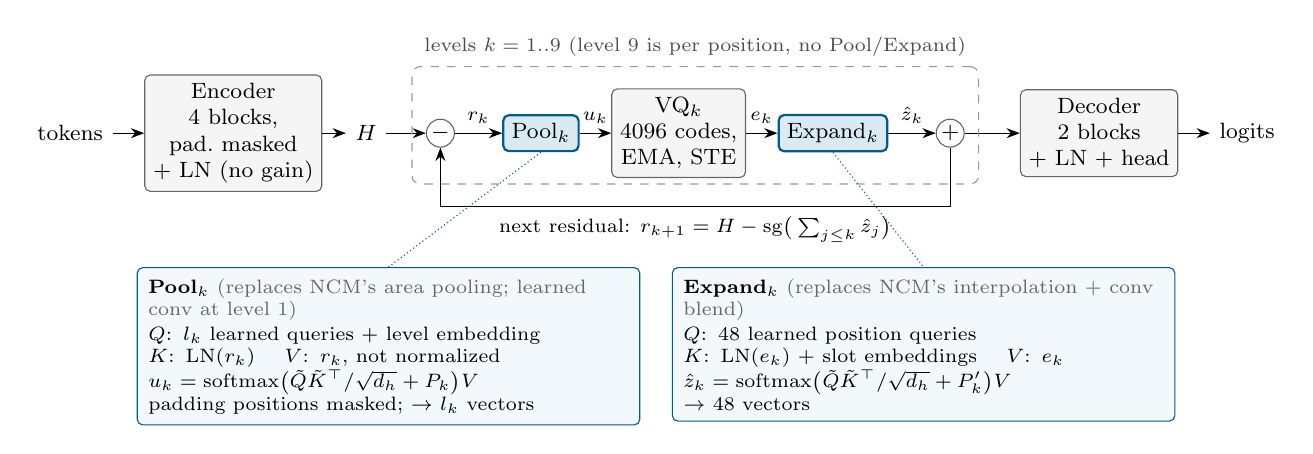
\begin{tikzpicture}[font=\footnotesize, >=Stealth, node distance=4mm,
  box/.style={draw=black!60, rounded corners=2pt, align=center, inner sep=3pt, fill=gray!8},
  new/.style={box, fill=slotA!15, draw=slotA!80!black, thick},
  zoom/.style={draw=slotA!80!black, rounded corners=2pt, fill=slotA!5, align=left, inner sep=4pt, text width=6.1cm, font=\scriptsize},
  op/.style={draw=black!60, circle, inner sep=0.5pt, fill=white},
  every edge/.style={draw, ->}]
% main row
\node (in) {tokens};
\node[box, right=of in] (enc) {Encoder\\4 blocks,\\pad.\ masked\\+ LN (no gain)};
\node[right=3mm of enc] (H) {$H$};
\node[op, right=5mm of H] (minus) {$-$};
\node[new, right=6mm of minus] (pool) {Pool$_k$};
\node[box, right=of pool] (vq) {VQ$_k$\\4096 codes,\\EMA, STE};
\node[new, right=of vq] (exp) {Expand$_k$};
\node[op, right=6mm of exp] (plus) {$+$};
\node[box, right=7mm of plus] (dec) {Decoder\\2 blocks\\+ LN + head};
\node[right=of dec] (out) {logits};
\draw[->] (in) -- (enc);
\draw[->] (enc) -- (H);
\draw[->] (H) -- (minus);
\draw[->] (minus) -- node[above, font=\scriptsize] {$r_k$} (pool);
\draw[->] (pool) -- node[above, font=\scriptsize] {$u_k$} (vq);
\draw[->] (vq) -- node[above, font=\scriptsize] {$e_k$} (exp);
\draw[->] (exp) -- node[above, font=\scriptsize] {$\hat z_k$} (plus);
\draw[->] (plus) -- (dec);
\draw[->] (dec) -- (out);
% residual feedback: r_{k+1} = H - sg(sum_{j<=k} zhat_j)
\draw[->] (plus.south) -- ++(0,-0.75) -| node[pos=0.25, below, font=\scriptsize] {next residual: $r_{k+1}=H-\mathrm{sg}\big(\sum_{j\le k}\hat z_j\big)$} (minus.south);
% loop frame
\node[draw=black!40, dashed, rounded corners=3pt, fit=(minus)(pool)(vq)(exp)(plus), inner sep=5pt, yshift=1mm,
      label={[font=\scriptsize, text=black!70]above:{levels $k=1..9$ (level 9 is per position, no Pool/Expand)}}] (loop) {};
% zoom-ins
\path (in.west) -- (out.east) coordinate[midway] (mid);
\node[zoom, anchor=north east] (zp) at ($(mid)+(-2mm,-17mm)$) {%
  \textbf{Pool$_k$} \textcolor{black!60}{(replaces NCM's area pooling; learned conv at level 1)}\\[1pt]
  $Q$: $l_k$ learned queries + level embedding\\
  $K$: LN$(r_k)$ \quad $V$: $r_k$, not normalized\\
  $u_k=\mathrm{softmax}\big(\tilde Q\tilde K^{\top}/\sqrt{d_h}+P_k\big)V$\\
  padding positions masked; $\to$ $l_k$ vectors};
\node[zoom, anchor=north west] (ze) at ($(mid)+(2mm,-17mm)$) {%
  \textbf{Expand$_k$} \textcolor{black!60}{(replaces NCM's interpolation + conv blend)}\\[1pt]
  $Q$: 48 learned position queries\\
  $K$: LN$(e_k)$ + slot embeddings \quad $V$: $e_k$\\
  $\hat z_k=\mathrm{softmax}\big(\tilde Q\tilde K^{\top}/\sqrt{d_h}+P'_k\big)V$\\
  $\to$ 48 vectors};
\draw[slotA!80!black, densely dotted] (pool.south) -- (zp.north);
\draw[slotA!80!black, densely dotted] (exp.south) -- (ze.north);
\end{tikzpicture}}
\caption{The T1 (CruxTok) tokenizer. Blue boxes replace NCM's per-level pooling and expansion; the residual loop, codebooks and nested dropout follow NCM. Section~\ref{sec:method} lists the other differences from the baselines (encoder and decoder depth, padding masking, loss terms, code restarts). In both attention blocks (linear projections omitted), $\tilde Q,\tilde K$ are RMS-normalized per head (QK-norm, \S\ref{sec:stability}) and $P_k$, $P'_k$ are learnable priors initialized to NCM's windows (Figure~\ref{fig:pooling}). Pooling values are the raw residual, so $u_k$ keeps the residual's scale, which shrinks with level. LN: LayerNorm; sg: stop-gradient. During training the decoder receives the sum up to a randomly truncated level (nested dropout).}
\label{fig:arch}
\end{figure}

\paragraph{Learned-query pooling (T1).} We call this tokenizer CruxTok, after the goal that its first level keep the crux of a sentence; the code and checkpoints use that name. Figure~\ref{fig:arch} shows the whole tokenizer. A transformer encoder (4 blocks, $d{=}384$, 6 heads) contextualizes the token embeddings, and its output passes through a LayerNorm without learned gain. At level $k$, $l_k$ learned queries cross-attend over the current residual with query--key--value attention \citep{vaswani2017attention}, as in PMA, Perceiver and Q-Former \citep{lee2019set,jaegle2021perceiver,li2023blip2}; G3PT uses the same down- and upsampling queries inside a multi-scale residual quantizer \citep{zhang2025g3pt}. Plain learned queries collapsed: every slot at a level pooled the same vector. We therefore add a learnable attention prior to the logits, a Gaussian bias as in \citet{yang2018localness}, initialized to centre on each of NCM's windows, so that slots start apart and can move (Figure~\ref{fig:pooling}a). For the reported runs the prior's sharpness is 1.0, chosen on held-out reconstruction in short pilot runs. At this sharpness the prior is wider than NCM's windows: at level~1 it spans 21.3 effective tokens against NCM's 12, with on average 75\% of its mass inside its own window. Expansion is the mirror image: $L$ learned position queries attend over the $l_k$ quantized vectors (with learned slot embeddings added to the keys) under their own learnable window prior. In both, keys are layer-normalized while values are not, so pooled vectors keep the residual's scale; pooling queries also carry a learned per-level embedding. Padding positions (NCM fills the window with EOS after the first EOS) are masked from the encoder's self-attention and from pooling attention; NCM masks no positions. The last level is quantized per position, as in NCM, and a 2-block decoder maps the summed reconstruction to token logits. We use a straight-through estimator \citep{bengio2013ste} at every level, with each residual detached from previous levels' quantized output.

\begin{figure}[t]
\centering
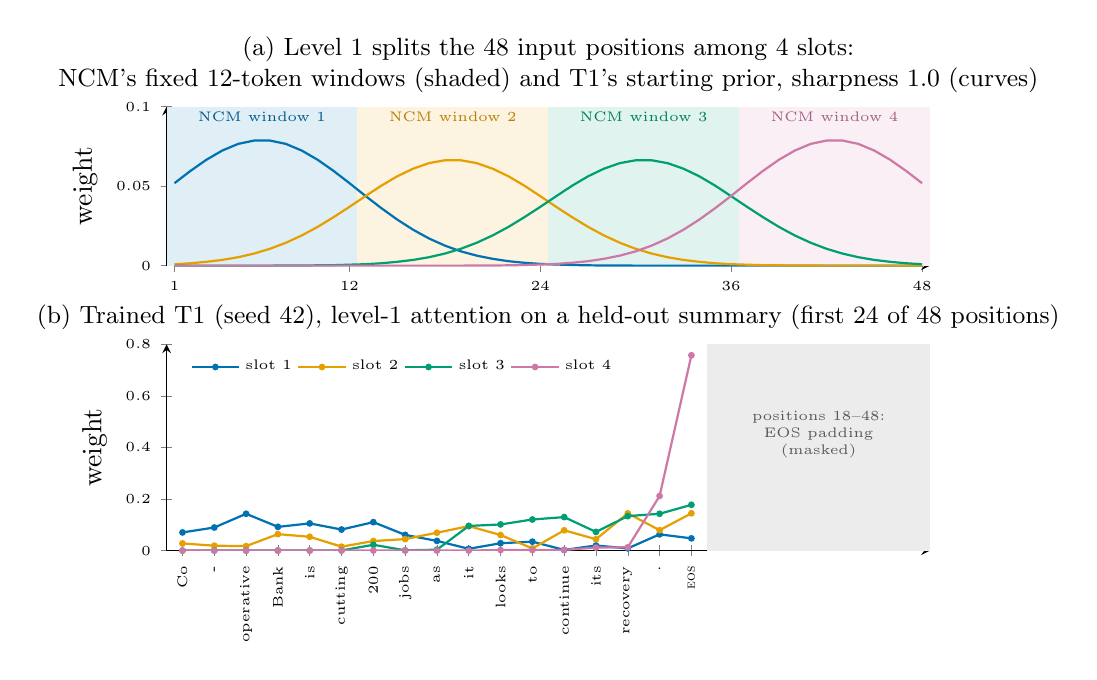
\begin{tikzpicture}
\begin{axis}[name=a, width=0.93\linewidth, height=3.6cm, xmin=0.5, xmax=48.5, ymin=0, ymax=0.10, ytick={0,0.05,0.1}, yticklabel style={/pgf/number format/fixed},
  xtick={1,12,24,36,48}, ylabel={weight}, yticklabel style={font=\tiny}, xticklabel style={font=\tiny},
  title={(a) Level 1 splits the 48 input positions among 4 slots:\\NCM's fixed 12-token windows (shaded) and T1's starting prior, sharpness 1.0 (curves)},
  title style={yshift=-1ex, align=center, font=\small}, axis lines=left, clip=false]
\fill[slotA!12] (axis cs:0.5,0) rectangle (axis cs:12.5,0.10);
\node[font=\tiny,slotA!80!black] at (axis cs:6.5,0.094) {NCM window 1};
\fill[slotB!12] (axis cs:12.5,0) rectangle (axis cs:24.5,0.10);
\node[font=\tiny,slotB!80!black] at (axis cs:18.5,0.094) {NCM window 2};
\fill[slotC!12] (axis cs:24.5,0) rectangle (axis cs:36.5,0.10);
\node[font=\tiny,slotC!80!black] at (axis cs:30.5,0.094) {NCM window 3};
\fill[slotD!12] (axis cs:36.5,0) rectangle (axis cs:48.5,0.10);
\node[font=\tiny,slotD!80!black] at (axis cs:42.5,0.094) {NCM window 4};
\addplot[slotA, thick, no marks] coordinates {(1,0.0519) (2,0.0596) (3,0.0666) (4,0.0724) (5,0.0766) (6,0.0787) (7,0.0787) (8,0.0766) (9,0.0724) (10,0.0666) (11,0.0596) (12,0.0519) (13,0.0439) (14,0.0362) (15,0.0290) (16,0.0226) (17,0.0171) (18,0.0126) (19,0.0090) (20,0.0063) (21,0.0043) (22,0.0028) (23,0.0018) (24,0.0011) (25,0.0007) (26,0.0004) (27,0.0002) (28,0.0001) (29,0.0001) (30,0.0000) (31,0.0000) (32,0.0000) (33,0.0000) (34,0.0000) (35,0.0000) (36,0.0000) (37,0.0000) (38,0.0000) (39,0.0000) (40,0.0000) (41,0.0000) (42,0.0000) (43,0.0000) (44,0.0000) (45,0.0000) (46,0.0000) (47,0.0000) (48,0.0000)};
\addplot[slotB, thick, no marks] coordinates {(1,0.0009) (2,0.0015) (3,0.0024) (4,0.0036) (5,0.0053) (6,0.0076) (7,0.0106) (8,0.0144) (9,0.0190) (10,0.0244) (11,0.0305) (12,0.0370) (13,0.0437) (14,0.0503) (15,0.0562) (16,0.0610) (17,0.0645) (18,0.0663) (19,0.0663) (20,0.0645) (21,0.0610) (22,0.0562) (23,0.0503) (24,0.0437) (25,0.0370) (26,0.0305) (27,0.0244) (28,0.0190) (29,0.0144) (30,0.0106) (31,0.0076) (32,0.0053) (33,0.0036) (34,0.0024) (35,0.0015) (36,0.0009) (37,0.0006) (38,0.0003) (39,0.0002) (40,0.0001) (41,0.0001) (42,0.0000) (43,0.0000) (44,0.0000) (45,0.0000) (46,0.0000) (47,0.0000) (48,0.0000)};
\addplot[slotC, thick, no marks] coordinates {(1,0.0000) (2,0.0000) (3,0.0000) (4,0.0000) (5,0.0000) (6,0.0000) (7,0.0000) (8,0.0001) (9,0.0001) (10,0.0002) (11,0.0003) (12,0.0006) (13,0.0009) (14,0.0015) (15,0.0024) (16,0.0036) (17,0.0053) (18,0.0076) (19,0.0106) (20,0.0144) (21,0.0190) (22,0.0244) (23,0.0305) (24,0.0370) (25,0.0437) (26,0.0503) (27,0.0562) (28,0.0610) (29,0.0645) (30,0.0663) (31,0.0663) (32,0.0645) (33,0.0610) (34,0.0562) (35,0.0503) (36,0.0437) (37,0.0370) (38,0.0305) (39,0.0244) (40,0.0190) (41,0.0144) (42,0.0106) (43,0.0076) (44,0.0053) (45,0.0036) (46,0.0024) (47,0.0015) (48,0.0009)};
\addplot[slotD, thick, no marks] coordinates {(1,0.0000) (2,0.0000) (3,0.0000) (4,0.0000) (5,0.0000) (6,0.0000) (7,0.0000) (8,0.0000) (9,0.0000) (10,0.0000) (11,0.0000) (12,0.0000) (13,0.0000) (14,0.0000) (15,0.0000) (16,0.0000) (17,0.0000) (18,0.0000) (19,0.0000) (20,0.0001) (21,0.0001) (22,0.0002) (23,0.0004) (24,0.0007) (25,0.0011) (26,0.0018) (27,0.0028) (28,0.0043) (29,0.0063) (30,0.0090) (31,0.0126) (32,0.0171) (33,0.0226) (34,0.0290) (35,0.0362) (36,0.0439) (37,0.0519) (38,0.0596) (39,0.0666) (40,0.0724) (41,0.0766) (42,0.0787) (43,0.0787) (44,0.0766) (45,0.0724) (46,0.0666) (47,0.0596) (48,0.0519)};
\end{axis}
\begin{axis}[at={(a.south west)}, anchor=north west, yshift=-1.0cm, width=0.93\linewidth, height=4.2cm,
  xmin=0.5, xmax=24.5, ymin=0, ymax=0.8, ylabel={weight}, yticklabel style={font=\tiny},
  xtick={1,...,17}, xticklabels={{Co},{-},{operative},{Bank},{is},{cutting},{200},{jobs},{as},{it},{looks},{to},{continue},{its},{recovery},{.},{\textsc{eos}}},
  xticklabel style={font=\tiny, rotate=90, anchor=east}, axis lines=left,
  title={\small (b) Trained T1 (seed 42), level-1 attention on a held-out summary (first 24 of 48 positions)},
  title style={yshift=-1ex}, legend style={font=\tiny, draw=none, at={(0.02,0.98)}, anchor=north west}, legend columns=4]
\fill[gray!15] (axis cs:17.5,0) rectangle (axis cs:24.5,0.8);
\node[font=\tiny, gray!70!black, align=center] at (axis cs:21,0.45) {positions 18--48:\\EOS padding\\(masked)};
\addplot[slotA, thick, mark=*, mark size=0.8pt] coordinates {(1,0.0703) (2,0.0894) (3,0.1427) (4,0.0919) (5,0.1053) (6,0.0815) (7,0.1102) (8,0.0608) (9,0.0374) (10,0.0068) (11,0.0284) (12,0.0345) (13,0.0024) (14,0.0197) (15,0.0084) (16,0.0629) (17,0.0473)};
\addlegendentry{slot 1}
\addplot[slotB, thick, mark=*, mark size=0.8pt] coordinates {(1,0.0277) (2,0.0188) (3,0.0172) (4,0.0637) (5,0.0534) (6,0.0151) (7,0.0368) (8,0.0444) (9,0.0692) (10,0.0948) (11,0.0603) (12,0.0082) (13,0.0786) (14,0.0439) (15,0.1445) (16,0.0789) (17,0.1446)};
\addlegendentry{slot 2}
\addplot[slotC, thick, mark=*, mark size=0.8pt] coordinates {(1,0.0000) (2,0.0000) (3,0.0000) (4,0.0000) (5,0.0000) (6,0.0003) (7,0.0224) (8,0.0009) (9,0.0033) (10,0.0955) (11,0.1013) (12,0.1205) (13,0.1298) (14,0.0722) (15,0.1336) (16,0.1427) (17,0.1775)};
\addlegendentry{slot 3}
\addplot[slotD, thick, mark=*, mark size=0.8pt] coordinates {(1,0.0000) (2,0.0000) (3,0.0000) (4,0.0000) (5,0.0000) (6,0.0000) (7,0.0000) (8,0.0000) (9,0.0000) (10,0.0000) (11,0.0020) (12,0.0018) (13,0.0026) (14,0.0114) (15,0.0127) (16,0.2117) (17,0.7577)};
\addlegendentry{slot 4}
\end{axis}
\end{tikzpicture}
\caption{Learned-query pooling at level~1. (a)~NCM pools four fixed 12-token windows. T1 has four learned queries whose attention starts from a Gaussian prior centred on those windows (sharpness 1.0), wider than the windows themselves. (b)~After training, on a held-out XSum summary drawn at random (seed 0) that fills 17 of the 48 positions: NCM's windows 3 and 4 would pool only EOS padding, while all four T1 slots attend to the text and none to padding. T1's slots are not confined to their windows: the prior is a soft bias, and padding is masked, so slots 3 and 4 spread onto the nearest text. Slot~4 puts most of its mass (0.76) on the first EOS.}
\label{fig:pooling}
\end{figure}

\paragraph{Objective.} The loss is token cross-entropy over the whole window plus, averaged over levels, NCM's terms $\beta\lVert z-\mathrm{sg}(\hat z_k)\rVert^2+\lVert\hat z_k-\mathrm{sg}(z)\rVert^2$ and a per-level commitment term $\beta\lVert u_k-\mathrm{sg}(e_k)\rVert^2$ that NCM does not use, with $\beta=0.25$. Here $u_k$ is the pooled residual, $e_k$ its codebook vector and $\hat z_k$ the reconstruction from levels $1..k$. T1's codebooks also restart codes whose usage falls below 1\% of uniform; NCM's do not.

\paragraph{Stabilizer.} Pooling and expansion attention use QK-normalization; Section~\ref{sec:stability} explains why.

\section{Experimental setup}
\paragraph{Training.} All tokenizers are trained on XSum training summaries \citep{narayan2018xsum} for 30{,}000 updates at batch 256, with AdamW (learning rate $5{\times}10^{-4}$ cosine-decayed to $5{\times}10^{-5}$, 1{,}000 warmup steps, $\beta_2{=}0.95$, weight decay 0.01, clipping at 1.0), EMA codebooks and nested dropout with probability 0.5. T1 accumulates two micro-batches of 128, so its EMA codebooks update twice per step and the nested-dropout level is drawn per micro-batch; T0-cap uses one batch of 256. This is about 16 times fewer sequences than NCM's tokenizer budget, so we compare only against NCM retrained under the same budget (T0-cap), never against the released checkpoint.

\begin{table}[t]
\centering
\footnotesize
\begin{tabular}{llrl}
\toprule
Run & Description & Params & Seeds \\
\midrule
T0-cap & NCM architecture and schedule, same budget & 60.6M & 42 (fp16), 2 (bf16) \\
T0-cap, matched & NCM with 5 encoder and 3 decoder blocks & 73.1M & 42, 2 (bf16) \\
T1 (CruxTok) & learned-query pooling & 73.2M & 42, 2 (bf16) \\
\bottomrule
\end{tabular}
\caption{Runs. Parameter counts include codebooks, following NCM. The fp16 and bf16 T0-cap runs do not differ significantly on PAWS or STS-B at any level.}
\label{tab:runs}
\end{table}

\paragraph{Code similarity.} The similarity of two sentences at level $k$ is the cosine between the means of their level $1..k$ codebook vectors. We report PAWS AUC \citep[labeled\_final test, 8{,}000 pairs;][]{zhang2019paws} and STS-B Spearman \citep[test, 1{,}379 pairs;][]{cer2017stsb}, both used for evaluation only. Differences use a paired bootstrap over pairs (2{,}000 resamples, 95\% CI). Floors are random scores, word Jaccard and TF-IDF cosine; the ceiling is all-mpnet-base-v2 \citep{reimers2019sbert}. A secondary measure averages the level-$k$ reconstruction over non-padding positions, since on STS-B the primary measure correlates with sentence length ($\rho$ with the shorter sentence's length between $-0.20$ and $-0.71$ across tokenizers at $k{=}1$--3, and $-0.63$ to $-0.71$ for T1) when most of the window is EOS filler.

\paragraph{Decodable meaning (protocol fixed before results).} We decode 1{,}000 random XSum test summaries from levels $1..k$ only. Measure A is the cosine between Qwen3-Embedding-8B embeddings of the original and its reconstruction, with a paired bootstrap over items. Measure B is a pairwise LLM judge \citep{zheng2023judge}: the judge sees the original and two reconstructions at the same $k$ and answers which keeps more of who, what, where and the outcome, ignoring fluency. Each item is judged in both orders, and a side wins only if both orders agree; win rate is (wins + ties/2)/$n$ with a bootstrap CI, where ties include order disagreements and $n$ counts the items with usable answers in both orders (991--1{,}000 of 1{,}000). Four candidate judges were scored on STS-B before use; we use GLM-5.3 with low reasoning effort (Spearman 0.897 with human scores, order consistency 0.94). One candidate, Kimi-K2.5, was excluded because 38\% of its answers were empty. In the $k{=}2$--3 runs against the matched baseline, unusable answers were asked once more with a larger token budget (1--8 answers per run). As a robustness check declared after the primary results, the runner-up Qwen3-235B-Instruct-2507 (Spearman 0.883, order consistency 0.915), which does not reason before answering, re-judges every comparison against the matched baseline with the same protocol.

\section{Results}
\subsection{Reconstruction}
\begin{table}[t]
\centering
\small
\begin{tabular}{lrrrr}
\toprule
Run & $k{=}1$ & $k{=}2$ & $k{=}3$ & Full \\
\midrule
T0-cap (s42 / s2) & 23.5 / 23.0 & 36.3 / 35.7 & 47.1 / 46.5 & 95.8 / 95.7 \\
T0-cap, matched (s42 / s2) & 19.3 / 19.6 & 32.3 / 32.3 & 45.6 / 45.6 & 97.8 / 97.9 \\
T1 (s42 / s2) & 23.5 / 24.4 & \pos{41.0 / 40.4} & \pos{60.1 / 60.7} & \pos{98.8 / 98.8} \\
\bottomrule
\end{tabular}
\caption{Token accuracy (\%) on the text tokens, including the first EOS, of the first 2{,}000 XSum validation summaries, decoding from levels $1..k$. Bold: T1 ahead of both baselines on both seeds.}
\label{tab:recon}
\end{table}

Table~\ref{tab:recon} shows that T1 reconstructs better than both baselines at every depth beyond level~1, by 13--15 points at $k{=}3$. Extra encoder and decoder depth in the matched baseline helps at full depth (95.8 to 97.8) but not at the coarse levels.

\subsection{Learned pooling puts more decodable meaning into level 1}\label{sec:decode}

\begin{figure}[t]
\centering
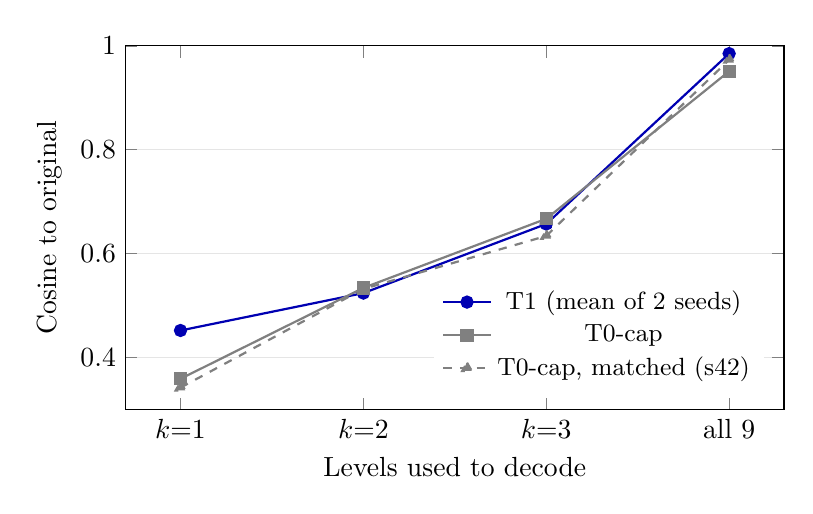
\begin{tikzpicture}
\begin{axis}[
  width=0.82\linewidth, height=6.2cm,
  xtick={1,2,3,4}, xticklabels={$k{=}1$,$k{=}2$,$k{=}3$,all 9},
  xlabel={Levels used to decode}, ylabel={Cosine to original},
  ymin=0.3, ymax=1.0, ymajorgrids, grid style={gray!20},
  legend style={at={(0.97,0.05)},anchor=south east,font=\small,draw=none},
  every axis plot/.append style={thick, mark size=2pt}]
\addplot[blue!70!black, mark=*, error bars/.cd, y dir=both, y explicit]
  coordinates {(1,0.452) +- (0,0.003) (2,0.524) +- (0,0.0035) (3,0.657) +- (0,0.0075) (4,0.985) +- (0,0.0005)};
\addlegendentry{T1 (mean of 2 seeds)}
\addplot[gray, mark=square*] coordinates {(1,0.359) (2,0.534) (3,0.667) (4,0.951)};
\addlegendentry{T0-cap}
\addplot[gray, dashed, mark=triangle*] coordinates {(1,0.342) (2,0.532) (3,0.634) (4,0.973)};
\addlegendentry{T0-cap, matched (s42)}
\end{axis}
\end{tikzpicture}
\caption{Measure A: embedding cosine between 1{,}000 XSum test summaries and their reconstructions from levels $1..k$. Error bars span the two T1 seeds and are mostly smaller than the markers. The second seed of the matched baseline is within 0.003 of seed 42 at every $k$.}
\label{fig:embed}
\end{figure}

\begin{table}[t]
\centering
\footnotesize
\begin{tabular}{lcccc}
\toprule
& $k{=}1$ & $k{=}2$ & $k{=}3$ & Full \\
\midrule
\multicolumn{5}{l}{\emph{Measure A: embedding cosine difference}} \\
T1 s42 $-$ T0-cap & \pos{+0.090} & $-$0.006 & $-$0.002 & \pos{+0.034} \\
T1 s2 $-$ T0-cap & \pos{+0.097} & \pos{$-$0.013} & \pos{$-$0.017} & \pos{+0.033} \\
T1 s42 $-$ T0-cap, matched & \pos{+0.107} & $-$0.004 & \pos{+0.031} & \pos{+0.012} \\
T1 s2 $-$ T0-cap, matched & \pos{+0.113} & \pos{$-$0.011} & \pos{+0.016} & \pos{+0.011} \\
\midrule
\multicolumn{5}{l}{\emph{Measure B: LLM-judge win rate, GLM-5.3}} \\
T1 s42 vs T0-cap & \pos{0.700} [0.678, 0.722] & 0.489 [0.463, 0.516] & \pos{0.541} [0.515, 0.568] & -- \\
T1 s42 vs T0-cap, matched & \pos{0.740} [0.720, 0.760] & 0.519 [0.493, 0.547] & \pos{0.637} [0.611, 0.663] & -- \\
T1 s2 vs T0-cap, matched & \pos{0.772} [0.753, 0.792] & 0.479 [0.452, 0.506] & \pos{0.592} [0.565, 0.618] & -- \\
\midrule
\multicolumn{5}{l}{\emph{Measure B: second judge, Qwen3-235B-Instruct-2507}} \\
T1 s42 vs T0-cap, matched & \pos{0.581} [0.563, 0.599] & \pos{0.545} [0.521, 0.567] & \pos{0.677} [0.654, 0.701] & -- \\
T1 s2 vs T0-cap, matched & \pos{0.607} [0.590, 0.625] & 0.498 [0.476, 0.521] & \pos{0.652} [0.627, 0.677] & -- \\
\bottomrule
\end{tabular}
\caption{Decodable meaning on 1{,}000 XSum test summaries. Both baselines are seed 42; results against the matched baseline's seed 2 are in the text. Bold: 95\% CI excludes 0 (measure A) or 0.5 (measure B). Measure-A CI half-widths are at most 0.009.}
\label{tab:decode}
\end{table}

Figure~\ref{fig:embed} and Table~\ref{tab:decode} show the main positive result. With four codes, T1 reconstructions are about 0.1 closer to the original in embedding space than either baseline, on both seeds. The judge agrees: T1's level-1 win rate is 0.70 against T0-cap, and 0.74 and 0.77 against the matched baseline. Counting outright preferences only, the judge picks T1 in 52\% of items against T0-cap (12\% for T0-cap), and in 57\% and 63\% against the matched baseline (9\% and 8\%); the rest are ties or order disagreements. The matched baseline is the weakest of the three at level~1, so the gain is not explained by parameter count. By $k{=}2$ the runs are within about 0.01 of each other in embedding space, and the judge finds T1 and the matched baseline about even (0.52 and 0.48). At $k{=}3$, T1 is ahead of the matched baseline again by both measures (judge 0.64 and 0.59), though not of the original T0-cap by measure A.

The second judge agrees in direction at every level but calls about twice as many ties, so its level-1 win rates are lower (0.58 and 0.61; outright, T1 in 26\% and 29\% of items and the baseline in 10\% and 8\%). Unlike the primary judge, it puts T1's largest margin at $k{=}3$ (0.68 and 0.65). The size of the level-1 effect is therefore judge-dependent; its sign is not.

A second seed of the matched baseline, trained after these results, gives the same picture. Its reconstructions are within 0.003 of seed 42's by measure A at every $k$ (no CI excludes 0). Against it, T1's level-1 win rates are 0.74 and 0.77 with GLM-5.3 and 0.58 and 0.60 with the second judge, and measure A rises by 0.105 and 0.111. At $k{=}3$ T1 stays ahead by both judges (0.63 and 0.58; 0.68 and 0.64) and by measure A ($+0.028$ and $+0.013$). At $k{=}2$ the runs are again about even, with one comparison now significant: GLM-5.3 puts T1 seed 2 behind (0.468 [0.443, 0.494]), as measure A already did ($-0.012$). In one of these runs 340 answers needed the second request, most likely because of failed API calls; 999 items were usable.

Table~\ref{tab:examples} shows reconstructions drawn at random. At level~1, T1 often preserves the type of event (an injured footballer, a crash at a racing championship) while getting names, places and numbers wrong, though on the boxing item it keeps little; the matched baseline's level~1 is mostly unrelated text, except on formulaic sentences such as the murder arrest.

\begin{table}[t]
\centering
\scriptsize
\begin{tabularx}{\linewidth}{>{\raggedright\arraybackslash}X>{\raggedright\arraybackslash}X>{\raggedright\arraybackslash}X}
\toprule
Original & T1, $k{=}1$ & T0-cap matched, $k{=}1$ \\
\midrule
West Ham striker Andy Carroll is facing up to six weeks out of action with a hamstring injury. & Newcastle midfielder Aaron Aaron has has he be surgery the out of the of after ankle injury. & Aales Minister Alex Johnson is preparing to his his. ahead of the. \\
\addlinespace
Michael Dunlop set the fastest times for the Ulster Grand Prix Superbike and Superstock classes in Thursday's delayed practice sessions at Dundrod. & A lorry driver who crashed been the crash at the World Tour Championships Championships in the the on Saturday the the Grand Grand in in in London. & When's of has a a to record for the second in a the of the- his, in England, the too on the years. \\
\addlinespace
A man has been arrested on suspicion of murder after a woman was found dead at a house in Worcestershire. & A man has been arrested on suspicion of murder after a woman woman was a in in in in indearkshire. & A man has been arrested on suspicion of murder after a woman- a murder at a house in arexhamhire. \\
\addlinespace
A former Welsh amateur boxing champion said she is turning professional as she does not have confidence in the governing body. & A former former assistant boss has has been been been described as as as of the the the the the election. & A man of David Cameron has said he will to the a\textquotedbl{} of a to hospital in the UK. \\
\bottomrule
\end{tabularx}
\caption{Level-1 reconstructions. Four of six items drawn uniformly at random (seed 0) from the 1{,}000 evaluated; the other two, and $k{=}3$ outputs, are in the repository.}
\label{tab:examples}
\end{table}

\paragraph{Do the queries choose tokens?} If pooling attention stayed on its starting prior, T1 would be close to NCM with extra parameters. On 256 held-out windows, pooling places zero mass on padding (44\% of positions), so we measure movement over text positions only, renormalizing both the attention and the starting prior. At levels 1--3, the attention on text differs from the starting prior by 37--53\% (total-variation distance per input, so this includes the between-input variation), the attention differs between inputs by 22--41\% (total-variation distance from the mean map), and it is narrower than the starting prior (14.6 vs 21.3 effective tokens at level~1, the prior counted over all 48 positions), though still wider than NCM's 12-token window. Both seeds agree within 0.04. The learned prior itself moves by only 0.05 at level~1, so the movement there comes from the queries. The starting prior is not the attention at initialization: with QK-normalization the query--key logits are already of order 1 at step 0, and we did not measure attention there. Figure~\ref{fig:pooling}b shows one example. Movement rules out fixed pooling; it does not show that attention moves toward meaning.

\subsection{Pooling does not organize the code space by meaning}\label{sec:geometry}
\begin{table}[t]
\centering
\footnotesize
\setlength{\tabcolsep}{3pt}
\resizebox{\linewidth}{!}{%
\begin{tabular}{lcccccc}
\toprule
& \multicolumn{3}{c}{PAWS AUC} & \multicolumn{3}{c}{STS-B Spearman} \\
\cmidrule(lr){2-4}\cmidrule(lr){5-7}
& $k{=}1$ & $k{=}2$ & $k{=}3$ & $k{=}1$ & $k{=}2$ & $k{=}3$ \\
\midrule
T0-cap (s42) & 0.546 & 0.549 & 0.551 & $-$0.058 & $-$0.029 & 0.067 \\
T0-cap, matched (s42 / s2) & 0.547 / 0.551 & \pos{0.571 / 0.573} & \pos{0.579 / 0.576} & $-$0.009 / \pos{0.026} & \pos{0.102 / 0.088} & \pos{0.282 / 0.280} \\
T1 (s42 / s2) & 0.551 / \pos{0.561} & 0.563 / 0.562 & 0.566 / 0.563 & $-$0.033 / 0.007 & $-$0.019 / $-$0.007 & 0.022 / 0.027 \\
\midrule
Floors: random / Jaccard / TF-IDF & \multicolumn{3}{c}{0.505 / 0.495 / 0.484} & \multicolumn{3}{c}{0.000 / 0.565 / 0.693} \\
Ceiling: all-mpnet-base-v2 & \multicolumn{3}{c}{0.652} & \multicolumn{3}{c}{0.834} \\
\bottomrule
\end{tabular}}
\caption{Code similarity, primary measure. Bold: best tokenizer in the column; both seeds of the matched baseline are bold where both are ahead of every other run. The two matched seeds do not differ significantly anywhere.}
\label{tab:geometry}
\end{table}

Decoding a sentence from its own codes and giving similar sentences similar codes are different properties. Table~\ref{tab:geometry} shows that the parameter-matched baseline is best at the second. Against it, T1 is behind at $k{=}2$--3 on both tasks and both seeds. The CIs exclude 0 everywhere except PAWS at $k{=}2$ ($-0.008$ [$-0.019$, $+0.003$] for both seeds). On STS-B at $k{=}3$ the gap is $-0.259$ [$-0.314$, $-0.208$] for seed 42 and $-0.255$ [$-0.311$, $-0.206$] for seed 2. At $k{=}1$, T1 is ahead on PAWS ($+0.004$ and $+0.014$; significant for seed 2 only), and STS-B is mixed ($-0.024$ and $+0.016$, neither significant). The padding-aware secondary measure agrees (STS-B at $k{=}3$: 0.257 for the matched baseline against 0.147 and 0.116 for T1). In absolute terms all tokenizers are weak sentence-similarity models: word Jaccard alone reaches 0.565 on STS-B, and on PAWS every tokenizer scores 0.55--0.58 on the primary measure against 0.65 for the sentence-encoder ceiling.

Against the matched baseline's second seed, STS-B at $k{=}2$--3 gives the same result ($k{=}3$: $-0.257$ and $-0.253$, CIs exclude 0). On PAWS at $k{=}2$--3 T1 is again behind by 0.010--0.014, significant only for seed 2 at $k{=}3$. At $k{=}1$, T1 seed 2's PAWS lead does not replicate ($+0.010$ [$-0.003$, $+0.024$]), and on STS-B T1 seed 42 is now significantly behind ($-0.059$ [$-0.121$, $-0.002$]). So the only coarse-level advantage of T1 in code similarity was not robust to the baseline's seed.

\section{Training stability}\label{sec:stability}
\paragraph{Attention-logit growth.} T1 diverged in bf16 under per-level STE. The expansion attention's query and key weights grew about 50-fold and its logits reached about $10^7$, the failure described by \citet{dehghani2023vit22b} and \citet{wortsman2024proxies}. RMS-normalizing queries and keys per head \citep{henry2020qknorm}, with the scale fixed so that the query--key term of the logits is bounded by $\sqrt{d_\text{head}}=8$ (the learned prior is added on top), removed the divergence.

\paragraph{A fallback that fails.} Applying STE only at the coarse levels, and NCM's global path below, left the deeper learned pools without a reconstruction gradient; their outputs collapsed to an RMS of 0.005. With learned pooling, every level needs its own gradient path.

\section{Limitations}\label{sec:limits}
The study uses one dataset of single-sentence summaries, a 48-token window and a reduced training budget; we do not show that attention moves toward meaning, only that it moves. No generator was trained, so whether a more decodable level~1 improves coarse-to-fine generation is untested; that is the main open question. Two earlier $k{=}3$ judge runs failed our 5\% missing-answer guard because the primary judge sometimes exhausted its token budget reasoning; the reported runs were made one at a time and passed it. The second judge was added after the primary results were known, and its API provider has scheduled it for retirement, so that check may not be repeatable there. Both judges are LLMs validated on STS-B sentence pairs, not on damaged reconstructions, and neither was checked against human judgments on this task. The matched baseline's second seed was trained after the primary results and is reported as a replication; the tables use seed 42 except where both are shown. Measure A partly rewards fluent reconstructions, which is why we pair it with the judge, which is told to ignore fluency.

\section{Conclusion}
Learned-query pooling makes the first four codes of a residual text tokenizer recover substantially more of a sentence than NCM's fixed pooling, including against an NCM with the same parameter count. It does not make similar sentences receive similar codes; a deeper NCM encoder does that better. For coarse-to-fine generation, the property that matters is likely decodability of the coarse levels, and that is the property pooling improves.

\paragraph{Reproducibility.} Code, configurations, evaluation outputs and the level-1 reconstructions used by the judge are at \url{https://github.com/Zilch123/CruxTok}. Trained tokenizers are at \url{https://huggingface.co/TimothDevA/cruxtok}.

\bibliographystyle{plainnat}
\bibliography{references}
\end{document}
